% Author: Kailash Ranganathan
% Email: kranganathan@berkeley.edu
% CSM16A Spring 2023



\qns{Capacitor Fundamentals}


\textbf{Learning Goal:} This problem aims to make students more familiar with the basics of capacitors by practicing the fundamental equations/concepts in application-based questions. 


\meta{
\begin{enumerate}
    \item The following questions are meant to develop a better intuition for both the inner workings/physics behind a capacitor as well as how capacitors function in circuits. 

    \item The idea of a capacitor can be hard to understand -- it's good to review what exactly a capacitor does in terms of storing opposite charges on its plates and inducing a voltage through the unequal distribution of charge. 

    \item First, ensure students understand the basic capacitor equations. These include $C = \frac{A \epsilon}{d}$, $Q = CV$, and $I = \frac{dQ}{dt}$. The difference between $\epsilon$ and $\epsilon_0$ should be clear too, where $\epsilon = \kappa \epsilon_0$.

    \item When reviewing it's useful to \textbf{think of $Q = CV$ as a definition (ie. to think of capacitance being defined by the amount of charge that can be stored per unit voltage)}. 

    \item The problems in these parts are, by themselves, mostly just computational, but it's the concepts that their results imply that are more significant (ie. in the capacitor charging paradox question or the dielectric breakdown section). If time permits, \textbf{a brief discussion of the significance of answer results would be very useful.}
\end{enumerate}


}

\begin{enumerate}

\item
Suppose we take two conducting disks of radius $r$ and place them a distance $2r$ from each other parallel to one another with air in between. \textbf{Calculate their capacitance in terms of $r$, $\epsilon_0$ (the permittivity of free space), and other constants.} \\ 
\ans{
    Here, we recognize that this is just a parallel-plate capacitor, for which the capacitance value is given by 
    \begin{align*}
        C = \frac{A \epsilon}{d}
    \end{align*}
    where $A$ is the area of the plates (or really, the area of overlap), $\epsilon$ is the dielectric constant of the medium between the capacitor plates, and $d$ is the distance between the plates. Here, we notice that $A = \pi r^2$, $d = 2r$, and $\epsilon = \epsilon_0$ for air, so the capacitance is just 
    \begin{align*}
        C = \frac{\pi r^2 \epsilon_0}{2r} = \boxed{\frac{\pi r \epsilon_0}{2}}
    \end{align*}
}

\itemA variable current source is hooked up to the ends of a capacitor as given by the following circuit. The current source emits a current as a function of time given by $i_s(t) = 200 \sin(\frac{\pi t}{1000})$, with $t$ given in seconds. Calculate the charge on the plates of the capacitor after $t_{\text{elapsed}} = 6000$ seconds. \emph{Hint: You do not need to know AC circuits to solve this question (that is 16B material)!} \\

\ans{
At first glance, this question might seem out of scope -- how are we supposed to calculate the charge over time of the capacitor without either knowing AC circuits or doing complex integrals? \\ \\
As a general problem-solving strategy, if a question seems completely out-of-scope, then there is probably some trick allowing us to simplify the question. Here, lets first think of the relationship between current and charge for capacitors, and then lets think about possibilities for simplifcation by looking at the current function. We know 
\begin{align*}
    I = \frac{dQ}{dt} \xrightarrow{} Q(t) = \int I(t) dt 
\end{align*}
If you haven't seen integrals, don't panic! Just think of this as a generalization of $Q(t) = I(t) \Delta t$ for when $I(t)$ is not constant over time. \\ 
Now, we have a clear expression for getting the charge as a function of current--integrate the current up till that time, and you've got the charge. But now lets think about our $i_s(t)$ -- a sine function oscillates from positive to negative symmetrically about the x-axis -- you can see its shape on the following graph. 
\begin{center}
    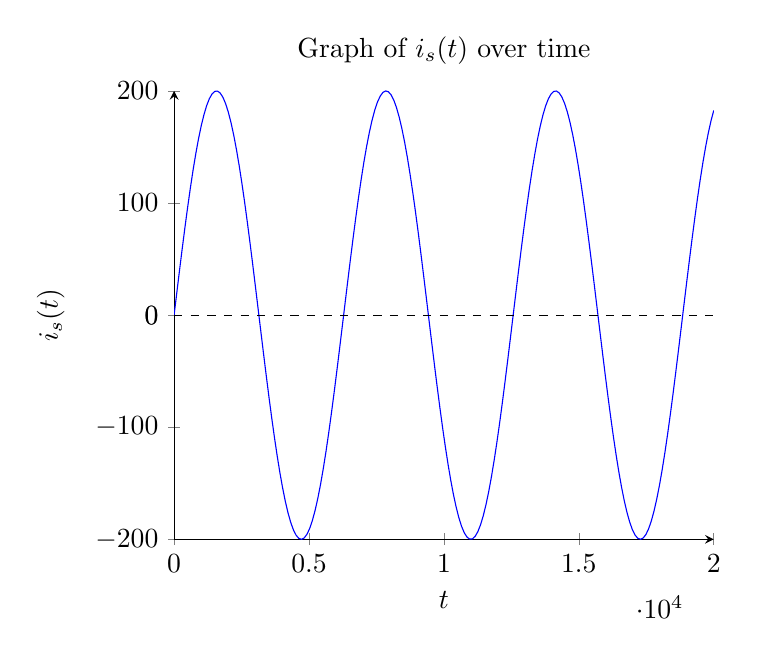
\begin{tikzpicture}
    \begin{axis}[axis lines = left, 
    xlabel = \(t\),
    ylabel = {\(i_s(t)\)},
    title = {Graph of $i_s(t)$ over time},
    grid style = dashed,
    extra y ticks = {0}
    ]
    \addplot[color=blue, domain=0:20000, samples = 200]{200*sin( deg(x)/1000)};
    \draw[dashed,thin] (axis cs: 0.1, 0 )-- (axis cs: 19988, 0);
    \end{axis}
    \end{tikzpicture}
\end{center}
We can note that the integral of $i_s(t)$ (the area under the current curve) basically cancels itself out every period, as the positive part annihilates the negative part perfectly. Thus, every period (which occurs every $t = 2000$ seconds, as we can see by the $\frac{\pi t}{1000}$ argument and the graph) the integral of $i_s(t) = 0$. As $t = 6000$ is a direct multiple of the $2000$ second-long period, $Q(6000) = \boxed{\int_0^{6000} i_s(t) dt = 0}$, as the sine function goes up and down exactly 3 times each, cancelling its area out completely. \\ \\
For those of you who are curious, the actual integral is given by 
\begin{align*}
    \int_0^{6000} 200 \sin(\frac{\pi t}{1000}) dt 
\end{align*}
which, if you solve using calculus (antiderivative of sine is cosine), will equation to zero. You'll learn more about this in 16B!
}

\meta{
The main important lesson of this question is to recognize that certain calculations that involve periodic elements can be "simplified" if the span of time given is a multiple of the period length (ie. if exactly $n$ periods have elapsed in the problem). This should also hopefully give students a little bit of intuition for how the charge actually changes as a function of current graphically, as integrals can be a bit confusing to think about. \\ \\ 
The last part, the exact calculation of the sine integral, is only necessary if students are still confused after the original explanation. 
}

\textbf{Charging Magic} \\
Suppose we have a circuit as given by the following:

\begin{center}
\begin{circuitikz}
\draw(0,0) 
	to[short] ++(3,0)
	to[C=$C_1$, v<=$ $] ++(0,3)
	to[opening switch=$t_1$] ++(-3, 0)
	to[short] ++(0,0)
	to[V=$V_s$] ++(0,-3);
	

\draw(3,0)
	to[short] ++(3,0)
	to[C=$C_2$, v<=$ $] ++(0,3)
	to[switch=$t_2$] ++(-3,0);
\draw (6, 0)
        to[short] node[ground] {} ++(0, 0);

\end{circuitikz}
\end{center}

Note the arrows of the switches -- At time $t_1$, the first switch opens to disconnect $V_S$ and $C_1$, and at time $t_2$, the second switch closes to connect $C_1$ and $C_2$ as given by the circuit diagram. 

\itemCalculate the total energy in the capacitors before time $t_1$. Assume that $C_2$ starts off as uncharged.

\ans{
Note that the total energy in the capacitors $E_{tot} = {E_C}_1 + {E_C}_2 = \frac{1}{2}C_1 V_1^2 + \frac{1}{2}C_2 V_2^2$

where the second equivalence is given by the definition of stored energy in capacitors. Specifically, we substitute $Q = CV$ into $E = \frac{QV}{2}$. Let's analyze the circuit at/before time $t_1$, when the left switch is closed. The circuit looks like the following: 

\begin{center}
\begin{circuitikz}
\draw(0,0) 
	to[short] ++(3,0)
	to[C=$C_1$, v<=$ $] ++(0,3)
	to[short] ++(-3, 0)
	to[short] ++(0,0)
	to[V=$V_s$] ++(0,-3);
	

\draw(3,0)
	to[short] ++(3,0)
	to[C=$C_2$, v<=$ $] ++(0,3)
	to[open] ++(-3,0);
\draw (6, 0)
        to[short] node[ground] {} ++(0, 0);

\end{circuitikz}
\end{center}
$C_2$ is connected to ground and nothing else, so we can disregard it in this phase (it's an open circuit route anyways, so no current/charge can flow into it). Thus, ${E_C}_2 = 0$ for before time $t_1$. For $C_1$, by KVL it's charged to a voltage of $V_S$, so ${E_C}_1 = \frac{1}{2}C_1 V_S^2$ for before time $t_1$. Hence, $\boxed{E_{tot} = \frac{1}{2}C_1 V_S^2}$. 

}


\itemAfter time $t_2$, calculate the new total energy in the capacitors. \emph{Hint: You may be tempted to say the energy is conserved as a shortcut, but the result may not be what you expect!} 

\ans{ Before we get into analyzing the new circuit, lets remember what's left over from the previous problem. The energy currently in $C_1$ is $\frac{1}{2}C_1 V_s^2$, and $C_2$ has no energy/is uncharged. Then, the new circuit is given by the following circuit (we just flip the switches from the previous circuit).

\begin{center}
\begin{circuitikz}
\draw(0,0) 
	to[short] ++(3,0)
	to[C=$C_1$, v<=$ $] ++(0,3)
	to[open] ++(-3, 0)
	to[short] ++(0,0)
	to[V=$V_s$] ++(0,-3);
	

\draw(3,0)
	to[short] ++(3,0)
	to[C=$C_2$, v<=$ $] ++(0,3)
	to[short] ++(-3,0);
\draw (6, 0)
        to[short] node[ground] {} ++(0, 0);

\end{circuitikz}
\end{center}
Now note that the voltage source is not connected to anything, so it is irrelevant for analysis. As $C_1$ and $C_2$ are now "in parallel," they must have the same voltage; that is, ${V_C}_1 = {V_C}_2 = \frac{Q_1}{C_1} = \frac{Q_2}{C_2}$. Here, we need to use charge sharing principles in order to figure out this common voltage. We know a node is created above the two capacitors, and thus the initial charge on $C_1$ must account wholly for the new distributed charges on both capacitors. That is, 
\begin{align*}
    {Q_C}_1 (t_1) = {Q_C}_1 (t_2) + {Q_C}_2(t_2)
\end{align*}
Because ${V_C}_1 = V_S$ before time $t_1$, and $Q = CV$ by definition, ${Q_C}_1 (t_1) = C_1 {V_C}_1 = C_1 V_S$. Hence, 

\begin{align*}
    C_1 V_S = {Q_C}_1 (t_2) + {Q_C}_2 (t_2)
\end{align*}
There are many ways we could go about solving this. The standard charge sharing way is to replace wither ${Q_C}_2$ for ${Q_C}_1$ or vice versa in the above equation and solve for the charges, but note that we're looking for energy on each capacitor, so all we need is their common voltage. Thus, lets write ${Q_C}_1 = C_1 V_C, {Q_C}_2 = C_2 V_C$, where $V_C = {V_C}_1 = {V_C}_2$, their common voltage in phase 2. Then, 
\begin{align*}
    C_1 V_S = C_1 V_C + C_2 V_C \xrightarrow{} V_C = \frac{C_1 V_S}{C_1 + C_2}
\end{align*}
Then, we can just apply $E = \frac{1}{2}CV^2$ to both capacitors. 
\begin{align*}
    {E_C}_1 = \frac{1}{2}C_1 V_C^2 = \frac{1}{2}C_1 (\frac{C_1 V_S}{C_1 + C_2})^2 = \frac{C_1}{2}\frac{C_1^2 V_S^2}{(C_1 + C_2)^2} \\ 
    {E_C}_2 = \frac{1}{2}C_2 V_C^2 = \frac{1}{2}C_2 (\frac{C_1 V_S}{C_1 + C_2})^2 = \frac{C_2}{2}\frac{C_1^2 V_S^2}{(C_1 + C_2)^2} \\ 
    E_{tot} = {E_C}_1 + {E_C}_2 = \frac{C_1}{2}\frac{C_1^2 V_S^2}{(C_1 + C_2)^2}  + \frac{C_2}{2}\frac{C_1^2 V_S^2}{(C_1 + C_2)^2} = \boxed{\frac{C_1^2V_S^2}{2(C_1 + C_2)}} 
\end{align*}
Note that $C_1 + C_2 > C_1$ as long as $C_2$ has a non-zero capacitance (ie. always), and so this energy is actually less than our energy from before! 
}

\itemSuppose $C_1 = C_2 = C$. Then, calculate the difference in energy between $t_1$ and $t_2$. (\emph{Optional: Nowhere in this question did we ever talk about resistance or the non-idealness of any element, and we can safely assume this circuit is a closed system. How can the energies at two times be different? Hint: Think about what we're doing when we close the second switch.})

\ans{
The differnce in energy is given by $E_{tot2} - E{tot1}$. For $C_1 = C_2 = C$, this is 
\begin{align*}
    \Delta E  = \frac{C^2V_S^2}{2(C + C)} - \frac{1}{2}C V_S^2  = \frac{1}{4} C V_S^2 - \frac{1}{2}C V_S^2 = \boxed{- \frac{1}{4}C V_S^2}
\end{align*}
In the previous problem, we hinted at the fact that the second timestep's total energy is smaller than the first, but here we clearly see that $\Delta E$ is \textit{negative} and that energy is lost somehow (moreover, the final energy is actually \textit{half} the initial energy). \\ \\
The reasoning behind this loss of energy is actually quite subtle. It turns out that when we close the second switch, this actually creates an impossible circuit. The closing of the second switch connects a capacitor at voltage $V_S$ to a capacitor that's uncharged (ie. $v = 0$). This puts two unequal voltages at the same node, which we know is a contradiction. There are two ways to "resolve" this paradox. \\
\begin{enumerate}
    \item The first way, which isn't really a resolution, is to assume that an infinite current flows between the capacitors to "instantaneously" resolve the different-voltage problem in the top node of the capacitors. This, of course, isn't physically realizable and cannot actually happen. \\

    \item The second way, which is what we've implicitly done, is to assume that the currents are finite and that charges can flow like they would in a normal circuit -- that is, to connect the capacitors at different voltages and have them eventually reach an equilibrium state, we have to implicitly act as if the process takes non-zero time, which (as you'll learn in 16B), requires a resistance to exist between the capacitors. It turns out no matter the value of this resistor, in this scenario with equal capacitors, half the initial energy will \textit{always} be dissipated. 
\end{enumerate}}

\meta{
The computation for this problem is not too bad, but the important part is to emphasize the intuition behind the "paradox" that's created here to give students a better understanding of capacitor workings. Ensure they understand the key issues at play -- connecting two different voltages onto the same node, and the assumption of "idealness" that isn't actually possible. 
}
 \\ \\ 

\textbf{Dielectric Limits} \\
The parameter $\epsilon$ is called the "dielectric constant" of the capacitor and gives the maximum energy a certain medium (ie. air) can store in the form of an electric field. If the voltage in a region gets too big, however, a phenomenon known as "dielectric breakdown" occurs -- the space can no longer carry the huge electric field and breaks down into a pure conductor. \\ \\ 
For the following parts of this question, we'll introduce the following extra equation. Recall that a capacitor stores energy in the form of an electric field in between its plates. Specifically, for a capacitor charged at voltage $V$, 
\begin{align*}
    V = Ed
\end{align*}
where $E$ is the electric field strength between the plates to sustain that voltage, and $d$ is the inter-plate distance. Think of the dielectric breakdown as the maximum electric field strenght a capacitor can sustain, and thus the corresponding $V$ is the maximum voltage that can go across the terminals of the capacitor. 
Useful values: 
\begin{enumerate}
    \item Dielectric strength of air: $3 \text{MV/m}$ 
    \item $\epsilon_0 = 8.854 \times 10^{-12} F m^{-1}$
    \item Dielectric strength of teflon: $19.7 \text{MV/m}$
    \item $\kappa$ of teflon: 2.1
    \item 1 MV = $1 \times 10^6 V$
\end{enumerate}

\itemSuppose a manufacturer of parallel plate capacitors designs square plate-capacitors with side-length 5 cm and separation distance 2 cm.  If the space between the plates is filled with air, \textbf{calculate the maximum voltage the capacitor can be connected to before reaching dielectric breakdown, and the charge that this capacitor can support at that maximum voltage}. \emph{Hint: How does the maximum voltage correspond to the dielectric breakdown, and how does this translate into calculation?}

\ans{ 
We can break down (no pun intended!) the calculations for this problem into three parts. 
\begin{enumerate}
    \item Calculate the maximum voltage the capacitor can handle using dielectric strength 
    \item Calculate the capacitance using known values 
    \item Calculate the maximum charge the capacitor can hold using the previous two parts and $Q = CV$
\end{enumerate}
Lets get started! \\ \\ We're given that $V = Ed$ for a capacitor, so some maximum voltage must satisfy $V_{max} = E_{max} d$. Here, we can note that the dielectric strength represents the maximum electric field sustainable through that material, and using the given values above, solve for $V_{max}$ (another sort of sneaky way to get at this line of reasoning is to notice that $E$ has units of V/m, and so does dielectric strength, and hence by problem-solving intuition they're probably one and the same. But knowing the concepts is a much safer approach!) 
\begin{equation*}
    V_{max} = E_{\text{max for air}} d = (3 \text{MV/m}) (2 \text{cm}) = (3 \times 10^6 \text{V/m}) (2 \times 10^{-2} \text{m}) = 6 \times 10^4 \text{V} = \boxed{60 \text{kV}}
\end{equation*}
Thus, our capacitor can be connected to up to 60 kilovolts before breaking down. Next, lets calculate the capacitance. The capacitance is given by 
\begin{align*}
    C = \frac{A \epsilon_0}{d} = \frac{(5 cm)^2 (8.854 \times 10^{-12} F m^{-1})}{2 cm} = \frac{25 \times 10^{-4} \text{m} \times 8.854 \times  p F}{2 \times 10^{-2} m} = 1.10675 pF
\end{align*}
where $1 pF = 10^{-12} F$. This part of the question is mostly just plugging in numbers, but make sure you get your units right! Also, remember because this capacitor is filled with air in the middle, we use $\epsilon = \epsilon_0$. Finally, we can calculate the maximum charge the capacitor can support under its maximum voltage. 
\begin{align*}
    Q_{max} = C V_{max} = 1.10675 pF \times 6 \times 10^4 V = 6.6405 \times 10^4 \times 10^{-12} C = \boxed{0.066405 \mu C}
\end{align*} 
}

\meta{
The calculations in this question are not really new and are just review of how to do capacitor problems. The only addition is the concept of dielectric breakdown, which the students should understand on a high-level without getting into the details of electromagnetism -- that different mediums have different capacities of holding electric field energy, which affect the functioning of capacitors. 
}

\itemNow, all other factors constant, suppose the space between the capacitor plates is replaced with teflon. Calculate the new maximum voltage the capacitor can be connected to before reaching dielectric breakdown, and interpret your result. \\
\ans{
We follow the exact same logic as in the previous part. Firstly, 
\begin{align*}
    V_{max} = E_{\text{max for teflon}}d = (19.7 \text{MV/m})(2 \text{cm}) = (19.7 \times 10^6 \text{V/m})(2 \times 10^{-2} \text{m}) = 39.4 \times 10^4 \text{V} = \boxed{394 \text{kV}}
\end{align*}
Already, we can see that this capacitor's breakdown voltage is much higher than the one with air between its plates. Next, lets calculate the capacitance. Remember because teflon is our new inter-plate medium, we need to use a different $\epsilon = \kappa_{\text{teflon}} \epsilon_0$ 
\begin{align*}
    C = \frac{A \epsilon}{d} = \frac{\kappa A \epsilon_0}{d} = \frac{2.1 \times A \epsilon_0}{d}
\end{align*}
Here, we can notice that $\frac{A \epsilon_0}{d}$ is just the capacitance we calculated in the last section, so we get 
\begin{align*}
    C_{\text{teflon}} = 2.1 C_{\text{air}} = 2.1 \times 1.10675 pF = 2.324 pF
\end{align*}
Lastly, we can calculate the new maximum charge the teflon capacitor can support. 
\begin{align*}
    Q_{max} = C V_{max} = 2.324 pF \times 394 kV = 2.324 \times 10^{-12} F \times 394 \times 10^3 V = \boxed{0.9157 \mu C}
\end{align*}
Note that this capacitor can support more than 10 times the charge of our previous "air capacitor." Hopefully this question gives a bit more insight into how while keeping the geometry of capacitors constant, different materials can bring out highly varied capacitor strengths and functionalities. 


}

\item(Optional) Suppose we had a pure insulator (no charge can move through it) and a pure conductor (charges move completely freely through it). Using the concepts from the previous part, calculate the dielectric constant $\epsilon$ for both materials. 

\ans{
This question is slightly tricky without a background in E\&M, but we can try to logic our way through. Lets start with the conductor as it's slightly more intuitive, and then move on to the insulator. \\ \\
Recall dielectric strength represents the capacity of a material to store energy in the electric field. What this means is that a material with a high dielectric strength is able to create large potential differences at small distances (because $V = Ed$). \\ \\ The key idea here is that these potential differences are only sustainable if the material can prevent the flow of current. Charges want to flow down voltage gradients to equalize the potential, so for a material to retain these large potential differences, it must be able to prevent the flow of charge. Thus, we can roughly correlate dielectric strength with how charge flows through a material. \\ \\
Now we can see how conductors/insulators connect to dielectric strength. Conductors allow free movement of charges, but this means they cannot retain any potential differences within them. If a conductor had a voltage $V$ across it, charges would instantly fall down that voltage difference and equalize it. This is why we sometimes model wires as having no voltage drop across them, regardless of how long they are. Thus, pure conductors can't store \textit{any} energy in electric fields and have \boxed{\text{0 dielectric strength, or $\epsilon = 0$}}. \\ \\
On the other hand, pure insulators prevent any flow of charge. So we could imagine that if we had a very large potential difference confined to a very small distance, a pure insulator would still prevent the flow of charges down this gradient and be able to preserve the potential difference. If charges cannot flow at all, we could theoretically pack an infinite voltage difference into a negligibly small difference, and thus pure insulators would have \boxed{\text{infinite dielectric strength, or $\epsilon = \infty$}}. 
\\ \\ 

\meta {In practice, the idea of dielectrics is a bit more subtle, but the above arguments roughly hold true. We can see why pure insulators cannot really exist (else we'd have materials with infinite electrical energy capacity). The \textbf{following analogy may be useful to give to students struggling to understand the concept of dielectric strength:} Preventing charges flowing down such a large potential difference in a small distance is akin to trying to hold a large amount of water at the top of a vertical pipe with some blocker. Eventually, the blocker will collapse due to the pressure and the water will go gushing through. Stronger blockers can hold more amounts of water at greater heights, but no blocker is infinitely strong. The same idea holds for dielectric strengths. }



}



\end{enumerate}